% !TEX root = ../Thesis.tex
\begin{document}
\documentclass[Thesis.tex]{subfiles}
\chapter{Fine-grained information presentation}
\label{ch:infpres}



%To be able to show or hide specific parts of the letters we try to break them apart into useful sections. (Irgendwie kein runder Übergang. Bin mir auch nicht ganz sicher, ob der nächste Teil noch in die Intro gehört. Macht aber schon Sinn, dann kann ich im nächsten Kapitel gleich mit einer Anwendung anfangen, für die ich alle anderen Methoden einführen muss.)
Many physician letters are rather long documents, spanning several pages. To increase the usability of a recommender system used in practice it is desirable to be able to show specific information like the diagnosis or the therapy history on demand or hide unnecessary parts of the letters like the introduction. It might also be desirable to compare letters only based on a specific section like therapy history. A first step towards this goal is the automatic extraction of the relevant paragraphs.



\section{Paragraph Extraction}

%As already mentioned above, the letters almost always contain separate
%paragraphs like greeting, diagnosis, therapy history and anamnesis.
%To be able to hide unnecessary information or to only present requested
%information it is useful to automatically extract individual
%paragraphs from the documents. 
The XML data format of the letters allows to automatize inspection of rather fine-grained structures present in the letters. One can automatically determine boldfaced characters for example. Because of this and because the documents are similar in structure, we use a rule based approach for extracting
the individual paragraphs. A simplified rule to find the beginning of the diagnosis paragraph is shown in pseudocode:
\bigskip

\begin{algorithm}[H]
	\DontPrintSemicolon
	diagnosisRegex = '[dD]iagnose(n)?'\;
	text = thisXmlNode.text()\;
	\If{regex.match(text, diagnosisRegex)
		$ {\bf and} $ boldface(text)
		$ {\bf and} $ precededByNewline(thisXmlNode)}{
		diagnosisStart = thisXmlNode\;
		}
		
%		\caption{Simplified pseudocode algorithm to find the beginning of the diagnosis paragraph}
\end{algorithm}
%		
%\bigskip
\bigskip

%\begin{lstlisting}
%diagnosis_regex = '[dD]iagnose(n)?'
%text = this_xml_node.text()
%if diagnosis_regex.match(text)
%	and boldface(text)
%	and preceded_by_newline(this_xml_node):
%then:
%	diagnosis_start = this_xml_node
%\end{lstlisting}

\bigskip
%(Weder der erste noch der zweite pseudocode gefällt mir bis jetzt. Wird noch geändert.)
\begin{figure}
	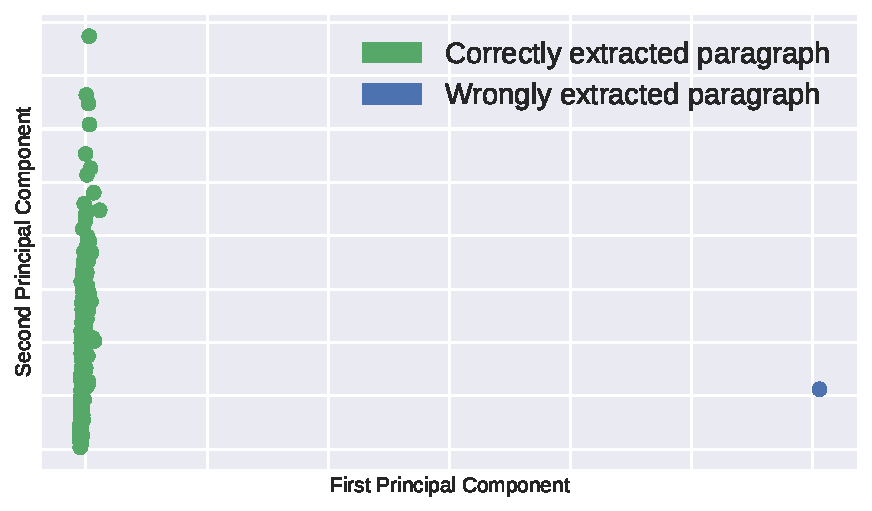
\includegraphics[width=\linewidth]{figures/bow_find_odd}
	\caption{2D PCA projection of bag of words representation of one incorrectly extracted diagnosis paragraph and several correctly extracted ones.}
	\label{fig:bow_find_odd}
\end{figure}
A regular expression is defined that matches the word diagnosis (the German word for diagnosis is "Diagnose").
The text of every node in the XML tree is checked for a regular expression match and whether it is boldfaced. If an XML node matches those criteria and is preceded by a newline, it is marked as the beginning of the diagnosis paragraph.
With a set of rules like the one above we automatically extract the
paragraphs of interest from the documents. This approach, however,
is not completely reliable, as the doctors are free to write the documents
in the way they please. Indeed we find several wrongly extracted paragraphs,
that e.g. include the subsequent paragraph as well. For our dataset
it is possible to check the extraction process by hand. However, this
is tedious work and is not scalable to bigger
datasets. We therefore explore whether we can in principle make use
of other automated methods to find paragraphs for which the rule based extraction
process does not produce desired results. We therefore take several correctly extracted and one incorrectly extracted
diagnosis paragraphs and convert them to their bag of words representation.
To get a feeling for how these vectors behave we use Principle Component
Analysis (PCA) to get a lower dimensional approximation of the vectors. PCA finds the linear
subspace with desired dimensionality of the original space that preserves as much of the variance of the vectors in the original space as possible. Thereby one can gain a low dimensional approximation of the high dimensional data and use this approximation for visual inspection.
See figure \ref{fig:bow_find_odd} for a 2D PCA plot of the bag of words representation
of the correctly and incorrectly extracted diagnosis paragraph. As is apparent from the figure, it would not be a
hard task to automatically detect the outlier. In this case the incorrectly
extracted paragraph includes not only the diagnosis, but also the
therapy history. In cases like this with additional text present, it is an easy task to
identify the incorrect ones. A harder problem arises, when only parts
of the paragraph of interest have been extracted. However, we believe
that this problem is of little concern, due to the way our rules are made.
%The way our rules are built it
%is very unlikely that we will face this problem. The paragraph would
%have to include an empty line, the subsequent one would have to contain
%only boldface characters and a few more conditions would have to be
%fulfilled for this problem to arise.
Indeed, we did not find a case
%of this problem in our dataset. (!correct! Ich könnte auch mal tatsächliche outlier detection machen, wenn du das für sinnvoll hälst. Hab ein paar Ideen, die gut funktionieren könnten, wollte aber keine Zeit rein stecken, falls wir es nicht benutzen wollen.)





\section{Paragraph Classification}
In our sample dataset, we can automate paragraph extraction as shown above. We can also detect for which paragraphs the procedure produces incorrect results. This approach works well only because the documents in our dataset generally adhere to a rough structure. For datasets from other clinics constructing a rule based extraction procedure is not only time consuming, it might not be possible at all. We therefore test an approach of classifying the extracted paragraphs into three categories---greeting, diagnosis and anamnesis. Our findings show that, surprisingly, this is not a hard problem. On unseen datasets it might therefore be possible to split text into unlabeled paragraphs with a basic rule based approach. One can possibly define a new paragraph to begin after a blank line and automatically label the resulting paragraphs with a predefined category. This way one would be able to hide or show specific information on demand even on datasets from other clinics.

We approach the problem again from a vector space based view-point. We compute the vector representation for every paragraph and use a classifier trained on these representations to predict the correct paragraph label. To get the best results we compare different text embedding methods. We test the standard bag of words, term frequency---inverse document frequency (tf-idf) and paragraph vector models. We also use Latent Semantic Analysis (LSA) and Latent Dirichlet Allocation (LDA) to get more condensed feature vector representations based on the tf-idf vector space. Before presenting the results of the different approaches we subsequently introduce these embedding methods.

\section*{Additional vector space models:}

\subsubsection*{Term Frequency---Inverse Document Frequency}

An extension of the bag of words model, that creates feature vectors based on term frequencies tf$(t,d)$ of term $t$ in document $d$ , is the term frequency---inverse document frequency model (tf-idf).
A common problem with the bag of words model is that some terms (even
after filtering stop words) appear often across texts in a corpus,
i.e. have a high term frequency, yet do not constitute a good feature
for discrimination between texts. Therefore a scaling factor for the
term frequencies is desired which captures the intuition that words
appearing often in a few texts but rarely in others are good discriminative
features for those texts. tf-idf refers to a specific scaling scheme, that downscales the
importance of frequent words, while upscaling the importance of rare
words. 

Term frequency tf$(t,d)$ usually refers to the standard word count.
Inverse document frequency idf$(t,C)$ of term $t$ and corpus $C$
can be computed as 
\[
\rm{idf}(t,C)=\log_{2}\left(\frac{|C|}{|\{d\in C:t\in d\}|}\right)
\]
where $|C|$ is the total number of documents in the corpus and $|\{d\in C:t\in d\}|$
is the number of documents in which term $t$ appears at least once.

Term frequency---Inverse document frequency tfidf$(t,d,C)$ is then
calculated as 
\[
\rm{tfidf}(t,d,C)=\rm{tf}(t,d)\cdot \rm{idf}(t,C)
\]


tf-idf can be used as a feature for the representation of the document
that is more robust to uninformative changes in the distribution of
common words and more expressive for rare words \citep{Manning2008vect}.


\subsubsection*{Latent Semantic Analysis}

An often occurring machine learning (ML) problem is that very high dimensional
feature vectors, as occurring in bag of words and tf-idf models,
tend to generalize poorly in subsequent tasks like classification.
In those cases it is desirable to have a more condensed lower dimensional
feature representation of documents that still captures most of the
variance in the bag of words representation. Latent semantic analysis
(LSA) of \citet{Deerwester1990} in its simplest form takes the plain bag of words
vectors of all documents in the corpus and constructs a term-document
matrix $\textbf{M}$, where $\textbf{M}[i,j]=\rm{tf}(t_{i},d_{j})$, i.e. row $i$ represents
the relation of term $i$ to all documents, while column $j$ represents
one document and the relation to all it's terms. So column j represents document $d_j$'s vector representation $\textbf{v}_{d_j}$.
\[ 
\begin{matrix} & \textbf{v}_{d_j}\\
& \downarrow\\
\textbf{v}_{t_i}^{T}\rightarrow & \begin{bmatrix}\rm{tf}(1,1) & \dots & \rm{tf}(1,|C|)\\
\vdots & \ddots & \vdots\\
\rm{tf}(|V|,1) & \dots & \rm{tf}(|V|,|C|)
\end{bmatrix}
\end{matrix}
\]
Singular value decomposition is then used on the term document matrix
$\textbf{M}$, allowing to find a $k$-dimensional ($k<dim(\textbf{M})$) linear subspace
of $\textbf{M}$, $\hat{\textbf{M}}$, that still captures as much of the original information
as possible, i.e. that captures as much of the variance in the original
space as possible. Column $j$ of $\hat{\textbf{M}}$ contains a $k$-dimensional,
approximate representation of the document j's feature vector $\textbf{v}_{d_{j}}$, called $\hat{\textbf{v}}_{d_{j}}$.
The document representations $\hat{\textbf{v}}_{d_j}$ in $\textbf{M}$'s linear subspace
spanned by $\hat{\textbf{M}}$ do no longer have an intuitive interpretation
as word counts, but can still be used as feature vectors for subsequent
ML tasks or can be analyzed for similarity. \citet{Deerwester1990} argue
that the resulting features have several appealing properties. The
LSA features can simply be viewed as a noise-reduced version of the
original features, but according to the original paper they can also
better deal with linguistic issues such as synonymy and polysemy.
This works because every original observation (i.e. document) is represented
as a linear combination of $k$ hidden (or latent) semantic concepts.
Terms that often appear together (i.e. are semantically related) will
then be mapped onto similar LSA representations and can thereby for
example capture some aspects of synonymy.

The value of $k$ is a parameter of the model and has to be specified
by the researcher. LSA can be used not only with the bag of words space as a basis, but also with the tf-idf space. Throughout this thesis we use LSA in the latter way.


\subsubsection*{Latent Dirichlet Allocation}

A popular probabilistic method for finding latent semantic features
of documents in a corpus is latent dirichlet allocation (LDA). As
with LSA the rationale is that it would be useful to find a shorter
or lower dimensional description for documents in the bag of words
vector space format for subsequent tasks. In the LDA context the latent
features are called topics and texts are represented as probabilistic
mixtures of these topics. A topic is represented by a probability
distribution over words and so a document is represented as a probabilistic
sample from several topic distributions over words. More specifically that means that documents in LDA space are represented by vectors of dimensionality $k$. The elements of one vector then represent the strength of association of the document with the respective topic. As in the case of LSA the
number of topics $k$ is a parameter and needs to be specified by
the researcher \citep{Blei2003}. 


\subsubsection*{Word Vectors}

In the standard bag of words model no relationship between words is
encoded, i.e. every word is dissimilar from every other word. Thereby
a lot of information is lost, as e.g. the words ``car'' and ``automobile''
are considered by the system to be as similar to each other as to
the word ``blue''. One way to encode relationships between words
is to embed them in a vector space. Just like the way document similarities
can be computed from their distances in the vector space model, similarities
of words can be computed, if the words are represented as vectors.
A first successful approach to this problem used the LSA model. Here
a single word can be represented as a pseudo document and thereby
be mapped into the LSA space. The resulting vector in the LSA feature
space can be considered a vector representation for the word and be
used for comparisons with other words \citep{Deerwester1990}.

\citet{Bengio2003} introduced a neural language model that uses
word vectors to predict subsequent words in a text and updates the
model as well as the vectors with gradient descent. It seems that
by being useful for prediction of subsequent words, the vectors represent
statistical information about word contexts and capture meaning of
the words to some extent.

Recently \citet{Mikolov2013a} proposed their influential Word2Vec model.
This model utilizes a neural network for the prediction of word vectors,
given other nearby word vectors. However, the authors focused on the
refinement of the word vectors only and were able to simplify the
net substantially, while gaining word vector ``performance'' (i.e.
vectors that perform better on a task designed to measure how well
the vectors capture human intuitions about the words). Their model
works simply with scalar products of input and output word vectors
(it has two vectors per word) and a softmax output layer for normalization.
This model comes in two architectural types: ``Continuous Bag of Words''
(CBOW) and ``Continuous Skip-gram'' (skip-gram). The former predicts
the output vector of a center word, given the $n$ previous and
$n$ subsequent input word vectors. The input vectors of the $2n$
surrounding words are averaged, the scalar product of this average
with every output word vector is computed and a softmax normalization
produces final output probabilities. The skip-gram model utilizes
the input vector of the center word to predict the output vectors
of surrounding words in a left and right context window of maximal
size $w$. The current window size $c$ is sampled uniformly from
range$(1,w)$ at every iteration. This results in $2c$ predictions
for every center word considered. The model parameters are updated
with gradient descent. After training, either only the input word vectors
or the input and output word vectors are used. In the latter case they are either averaged
or concatenated to produce the final word vectors used for subsequent
tasks. 

A note on computational cost: The softmax output layer is very inefficient
as it requires the computation of $|V|$ scalar products (every word
in the vocabulary). As a first speed up a hierarchical softmax \citep{Morin2005} is
used as an approximation to the real softmax, that reduces the number
of scalar product computations to $\log_{2}(|V|)$ \citep{Mikolov2013a}.
In a subsequent publication the authors introduced a
simplified variant of Noise Contrastive Estimation \citep{Gutmann2012}, called
Negative Sampling, that further reduces the computational complexity,
while still giving useful word vectors \citep{Mikolov2013b}. 

With these architecture and approximation simplifications the Word2Vec
model is able to train on a vast amount of text data (billions of
words) in a matter of hours. Mainly through those speed ups (and the concomitant larger amounts of processable data) word2vec is able to produce better word vectors, than previously possible.

\subsubsection*{Paragraph Vector---An extension of Word2Vec}

A simple extension of the word2vec model allows to obtain vectors
for sentences or longer passages of text. An additional vector is
introduced for every piece of text, that we regard as a separate entity
(a sentence, a paragraph or a document). This so called paragraph
vector is then used in two different ways in the extensions of CBOW
and skip-gram. In the Distributed Memory (DM) model, an extension
of CBOW, the paragraph vector is used in combination (average or concatenation)
with the vectors of surrounding words to predict a center word. In
the Distributed bag of words model, an extension of skip-gram, the
paragraph embedding is used to predict words randomly sampled from
the paragraph.

After the initial training phase a second step, called inference phase, is necessary to gain paragraph embeddings. A paragraph vector is initialized randomly, the rest of the model is kept fixed and the normal training procedure of word prediction and gradient descent on the paragraph vector is done. Thereby the final document embeddings are produced, which can be used like the embeddings of the methods described above. Note, however, that the time until the model reaches convergence both in the training and in the inference phase is unknown and a number of running epochs for both phases must be specified beforehand \citep{Le2014}.





\section*{Classification Results}

After having introduced the additional embedding methods tf-idf, LSA, LDA and paragraph vector, we now use their embeddings for classification of the paragraphs into respective categories. Therefore we take all the extracted greeting, diagnosis and anamnesis paragraphs and map them to one of the embedding representations. Then logistic regression is trained on a training portion of the dataset and the performance evaluated on a testing portion. As our dataset is relatively small we use leave-one-out cross-validation to be able to use every data point as test data. Thereby we obtain as much information about the performance as is possible with such limited data.

As vector embedding methods we test all methods described above. For LSA and LDA we tune the hyperparameter of dimensionality $k$ to obtain best results. The paragraph vector method has several rather unintuitive hyperparameters, that need tuning. We start with hyperparameters reported as working well in the literature \citep{Lau2016}. From there we use a randomized search strategy to find better fitting parameters for our specific problem. Results of our evaluation can be found in table \ref{table:para_class_acc}. Several things are noteworthy about the results. First it is surprisingly easy in general to use a small number of training paragraphs (less than 300 per category) to predict its label with very high accuracy. Second all methods are indeed outperformed by the more recent paragraph vector approach. However, the paragraph vector performance comes with the cost of needing to tune many hyperparameters, whose influence is not intuitively clear. Third LSA performance is always smaller or equal to tf-idf performance. As the tf-idf vector space has several thousand dimensions, but we only have several hundred texts, all these texts must fall into a linear subspace with dimension no greater than the number of texts. We assume the dimension is even substantially smaller, as LSA vectors produce the same results in classification accuracy when reducing the number of dimensions even much further.
\begin{table}[h]
	\begin{tabular}{|c||c|c|c|c|c|}
		\hline 
		Embedding Method & BOW & TF-IDF & LSA & LDA  & Para2Vec\tabularnewline
		\hline 
		\hline 
		Classification Accuracy & 0.995 & 0.997 & 0.997 & 0.992 & \underline{1.0}\tabularnewline
		\hline 
	\end{tabular}
	\caption{Mean paragraph classification accuracy of logistic regression measured with leave-one-out cross-validation for different vector embedding methods.}
	\label{table:para_class_acc}
\end{table}

To gain a more intuitive understanding of the performance of these approaches we use PCA to get a 2D approximation of the vectors of the extracted paragraphs. In figure \ref{fig:pv_tf_pca} one can compare the 2D PCA projections of the tf-idf and the paragraph vector models. While it is obvious that both methods can produce good results even just using a linear classifier, it is also easy to see that the paragraph vectors are easier separable (although not linearly separable in the 2D projection). We conclude that paragraph vector is the best suited method for this classification task. Additionally we note that it works surprisingly well with very limited training data.


\begin{figure}
	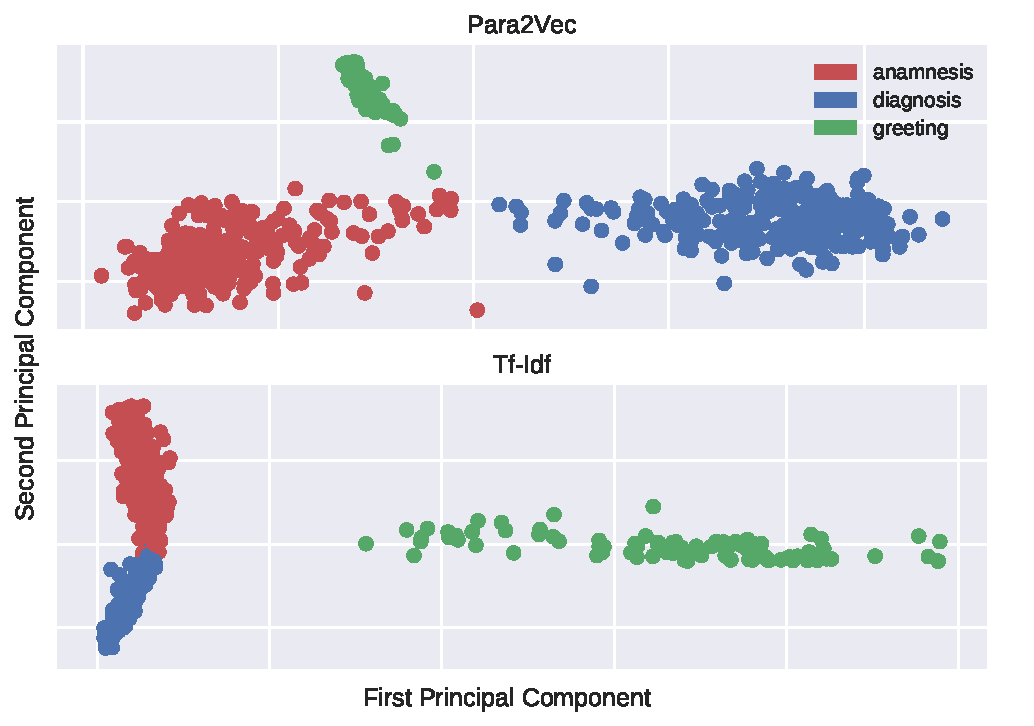
\includegraphics[width=\linewidth]{figures/para2vec_tfidf_pca}
	\caption{2D PCA projections of a vector space embedding of the physician letter paragraphs. Colors encode the respective paragraph category for each vector. \textbf{Top:} Paragraph vector space.  \textbf{Bottom:} Tf-idf vector space.}
	\label{fig:pv_tf_pca}
\end{figure}

\end{document}